%DIF 1c1
%DIF LATEXDIFF DIFFERENCE FILE
%DIF DEL tex_diff_tmp/supporting_information_old.tex   Mon Apr 27 23:44:58 2026
%DIF ADD supporting_information.tex                    Mon Apr 27 21:41:13 2026
%DIF < %%%%%%%%%%%%%%%%%%%%%%%%%%%%%%%%%%%%%%%%%%%%%%%%%%%%%%%%%%%%%%%%%%%%%
%DIF -------
%%%%%%%%%%%%%%%%%%%%%%%%%%%%%%%%%%%%%%%%%%%%%%%%%%%%%%%%%%%%%%%%%%%%% %DIF > 
%DIF -------
%% This is a (brief) model paper using the achemso class
%% The document class accepts keyval options, which should include
%% the target journal and optionally the manuscript type. 
%%%%%%%%%%%%%%%%%%%%%%%%%%%%%%%%%%%%%%%%%%%%%%%%%%%%%%%%%%%%%%%%%%%%%
\documentclass[journal=jacsat,manuscript=article]{achemso}

%%%%%%%%%%%%%%%%%%%%%%%%%%%%%%%%%%%%%%%%%%%%%%%%%%%%%%%%%%%%%%%%%%%%%
%% Place any additional packages needed here.  Only include packages
%% which are essential, to avoid problems later. Do NOT use any
%% packages which require e-TeX (for example etoolbox): the e-TeX
%% extensions are not currently available on the ACS conversion
%% servers.
%%%%%%%%%%%%%%%%%%%%%%%%%%%%%%%%%%%%%%%%%%%%%%%%%%%%%%%%%%%%%%%%%%%%%
\usepackage[version=3]{mhchem} % Formula subscripts using \ce{}
\usepackage{siunitx}
\usepackage{graphicx}
\usepackage{xr} % For cross-referencing equations from main.tex
\usepackage{multirow}
%DIF 20a20
\usepackage{lineno} %DIF > 
%DIF -------
\externaldocument{main}

%%%%%%%%%%%%%%%%%%%%%%%%%%%%%%%%%%%%%%%%%%%%%%%%%%%%%%%%%%%%%%%%%%%%%
%% If issues arise when submitting your manuscript, you may want to
%% un-comment the next line.  This provides information on the
%% version of every file you have used.
%%%%%%%%%%%%%%%%%%%%%%%%%%%%%%%%%%%%%%%%%%%%%%%%%%%%%%%%%%%%%%%%%%%%%
%%\listfiles

%%%%%%%%%%%%%%%%%%%%%%%%%%%%%%%%%%%%%%%%%%%%%%%%%%%%%%%%%%%%%%%%%%%%%
%% Place any additional macros here.  Please use \newcommand* where
%% possible, and avoid layout-changing macros (which are not used
%% when typesetting).
%%%%%%%%%%%%%%%%%%%%%%%%%%%%%%%%%%%%%%%%%%%%%%%%%%%%%%%%%%%%%%%%%%%%%
\newcommand*\mycommand[1]{\texttt{\emph{#1}}}
%DIF 35a36-37
\newcommand{\ChangeTagStart}[1]{\linelabel{changetag:start:#1}} %DIF > 
\newcommand{\ChangeTagEnd}[1]{\linelabel{changetag:end:#1}} %DIF > 
%DIF -------
\setcounter{figure}{0}
\renewcommand{\thefigure}{S\arabic{figure}}
\setcounter{table}{0}
\renewcommand{\thetable}{S\arabic{table}}

%% Counter for numbered subsection parts with Roman numerals
\newcounter{supppart}

\renewcommand{\thesupppart}{\Roman{supppart}}

\newcommand{\subsectionpart}[2]{%
  \refstepcounter{supppart}%
  \subsection{\thesupppart. #2}%
  \label{supppart:#1}%
}

\renewcommand{\bibsection}{\section*{Supporting References}}

%%%%%%%%%%%%%%%%%%%%%%%%%%%%%%%%%%%%%%%%%%%%%%%%%%%%%%%%%%%%%%%%%%%%%
%% Meta-data block
%% ---------------
%% Each author should be given as a separate \author command.
%%
%% Corresponding authors should have an e-mail given after the author
%% name as an \email command. Phone and fax numbers can be given
%% using \phone and \fax, respectively; this information is optional.
%%
%% The affiliation of authors is given after the authors; each
%% \affiliation command applies to all preceding authors not already
%% assigned an affiliation.
%%
%% The affiliation takes an option argument for the short name.  This
%% will typically be something like "University of Somewhere".
%%
%% The \altaffiliation macro should be used for new address, etc.
%% On the other hand, \alsoaffiliation is used on a per author basis
%% when authors are associated with multiple institutions.
%%%%%%%%%%%%%%%%%%%%%%%%%%%%%%%%%%%%%%%%%%%%%%%%%%%%%%%%%%%%%%%%%%%%%
\author{Haruya Ishida}
\affiliation[Kyushu University]
{Department of Aeronautics and Astronautics, Kyushu University, Nishi-Ku, Motooka 744, Fukuoka 819-0395, Japan}
\author{Koji Takahashi}
\affiliation[Kyushu University]
{Department of Aeronautics and Astronautics, Kyushu University, Nishi-Ku, Motooka 744, Fukuoka 819-0395, Japan}
\alsoaffiliation[I2CNER]
{International Institute for Carbon-Neutral Energy Research (WPI-I2CNER), Kyushu University, Nishi-Ku, Motooka 744, Fukuoka 819-0395, Japan}
\author{Vishwanath Ganesan}
\affiliation[UIUC MechSE]
%DIF 83c86
%DIF < {Department of Mechanical Science and Engineering, University of Illinois at Urbana-Champaign, Urbana, IL, USA}
%DIF -------
{Department of Mechanical Science and Engineering, University of Illinois at Urbana-Champaign, Urbana, IL 61801, USA} %DIF > 
%DIF -------
\author{Nenad Miljkovic}
\affiliation[I2CNER]
{International Institute for Carbon-Neutral Energy Research (WPI-I2CNER), Kyushu University, Nishi-Ku, Motooka 744, Fukuoka 819-0395, Japan}
\alsoaffiliation[UIUC MechSE]
%DIF 88c91
%DIF < {Department of Mechanical Science and Engineering, University of Illinois at Urbana-Champaign, Urbana, IL, USA}
%DIF -------
{Department of Mechanical Science and Engineering, University of Illinois at Urbana-Champaign, Urbana, IL 61801, USA} %DIF > 
%DIF -------
\alsoaffiliation[UIUC MRL]
%DIF 90c93
%DIF < {Materials Research Laboratory, University of Illinois at Urbana-Champaign, Urbana, IL, USA}
%DIF -------
{Materials Research Laboratory, University of Illinois at Urbana-Champaign, Urbana, IL 61801, USA} %DIF > 
%DIF -------
\alsoaffiliation[UIUC ECE]
%DIF 92c95
%DIF < {Department of Electrical and Computer Engineering, University of Illinois at Urbana-Champaign, Urbana, IL, USA}
%DIF -------
{Department of Electrical and Computer Engineering, University of Illinois at Urbana-Champaign, Urbana, IL 61801, USA} %DIF > 
%DIF -------
\alsoaffiliation[iSEE]
%DIF 94c97
%DIF < {Institute for Sustainability, Energy and Environment (iSEE), University of Illinois at Urbana-Champaign, Urbana, IL, USA}
%DIF -------
{Institute for Sustainability, Energy and Environment (iSEE), University of Illinois at Urbana-Champaign, Urbana, IL 61801, USA} %DIF > 
%DIF -------
\alsoaffiliation[ARC]
%DIF 96c99
%DIF < {Air Conditioning and Refrigeration Center, University of Illinois at Urbana-Champaign, Urbana, IL, USA}
%DIF -------
{Air Conditioning and Refrigeration Center, University of Illinois at Urbana-Champaign, Urbana, IL 61801, USA} %DIF > 
%DIF -------
\author{Hideaki Teshima}
\affiliation[Kyushu University]
{Department of Aeronautics and Astronautics, Kyushu University, Nishi-Ku, Motooka 744, Fukuoka 819-0395, Japan}
\email{hteshima05@aero.kyushu-u.ac.jp}
\alsoaffiliation[I2CNER]
{International Institute for Carbon-Neutral Energy Research (WPI-I2CNER), Kyushu University, Nishi-Ku, Motooka 744, Fukuoka 819-0395, Japan}

%%%%%%%%%%%%%%%%%%%%%%%%%%%%%%%%%%%%%%%%%%%%%%%%%%%%%%%%%%%%%%%%%%%%%
%% The document title should be given as usual. Some journals require
%% a running title from the author: this should be supplied as an
%% optional argument to \title.
%%%%%%%%%%%%%%%%%%%%%%%%%%%%%%%%%%%%%%%%%%%%%%%%%%%%%%%%%%%%%%%%%%%%%
\title[Title_supporting_information]
  {Supporting Information\\
  Water Does Not Slip on Hydrophobic Surfaces: Insights from Slip Length Mapping}

%%%%%%%%%%%%%%%%%%%%%%%%%%%%%%%%%%%%%%%%%%%%%%%%%%%%%%%%%%%%%%%%%%%%%
%% Some journals require a list of abbreviations or keywords to be
%% supplied. These should be set up here, and will be printed after
%% the title and author information, if needed.
%%%%%%%%%%%%%%%%%%%%%%%%%%%%%%%%%%%%%%%%%%%%%%%%%%%%%%%%%%%%%%%%%%%%%
\abbreviations{IR,NMR,UV}
\keywords{American Chemical Society, \LaTeX}

%%%%%%%%%%%%%%%%%%%%%%%%%%%%%%%%%%%%%%%%%%%%%%%%%%%%%%%%%%%%%%%%%%%%%
%% The manuscript does not need to include \maketitle, which is
%% executed automatically.
%%%%%%%%%%%%%%%%%%%%%%%%%%%%%%%%%%%%%%%%%%%%%%%%%%%%%%%%%%%%%%%%%%%%%
%DIF PREAMBLE EXTENSION ADDED BY LATEXDIFF
%DIF CFONT PREAMBLE %DIF PREAMBLE
\RequirePackage{color}\definecolor{RED}{rgb}{1,0,0}\definecolor{BLUE}{rgb}{0,0,1} %DIF PREAMBLE
\DeclareOldFontCommand{\sf}{\normalfont\sffamily}{\mathsf} %DIF PREAMBLE
\providecommand{\DIFadd}[1]{{\protect\color{blue} #1}} %DIF PREAMBLE
\providecommand{\DIFdel}[1]{} %DIF PREAMBLE
%DIF SAFE PREAMBLE %DIF PREAMBLE
\providecommand{\DIFaddbegin}{} %DIF PREAMBLE
\providecommand{\DIFaddend}{} %DIF PREAMBLE
\providecommand{\DIFdelbegin}{} %DIF PREAMBLE
\providecommand{\DIFdelend}{} %DIF PREAMBLE
\providecommand{\DIFmodbegin}{} %DIF PREAMBLE
\providecommand{\DIFmodend}{} %DIF PREAMBLE
%DIF FLOATSAFE PREAMBLE %DIF PREAMBLE
\providecommand{\DIFaddFL}[1]{\DIFadd{#1}} %DIF PREAMBLE
\providecommand{\DIFdelFL}[1]{} %DIF PREAMBLE
\providecommand{\DIFaddbeginFL}{} %DIF PREAMBLE
\providecommand{\DIFaddendFL}{} %DIF PREAMBLE
\providecommand{\DIFdelbeginFL}{} %DIF PREAMBLE
\providecommand{\DIFdelendFL}{} %DIF PREAMBLE
\newcommand{\DIFscaledelfig}{0.5}
%DIF HIGHLIGHTGRAPHICS PREAMBLE %DIF PREAMBLE
\RequirePackage{settobox} %DIF PREAMBLE
\RequirePackage{letltxmacro} %DIF PREAMBLE
\newsavebox{\DIFdelgraphicsbox} %DIF PREAMBLE
\newlength{\DIFdelgraphicswidth} %DIF PREAMBLE
\newlength{\DIFdelgraphicsheight} %DIF PREAMBLE
% store original definition of \includegraphics %DIF PREAMBLE
\LetLtxMacro{\DIFOincludegraphics}{\includegraphics} %DIF PREAMBLE
\newcommand{\DIFaddincludegraphics}[2][]{{\color{blue}\fbox{\DIFOincludegraphics[#1]{#2}}}} %DIF PREAMBLE
\newcommand{\DIFdelincludegraphics}[2][]{% %DIF PREAMBLE
\sbox{\DIFdelgraphicsbox}{\DIFOincludegraphics[#1]{#2}}% %DIF PREAMBLE
\settoboxwidth{\DIFdelgraphicswidth}{\DIFdelgraphicsbox} %DIF PREAMBLE
\settoboxtotalheight{\DIFdelgraphicsheight}{\DIFdelgraphicsbox} %DIF PREAMBLE
\scalebox{\DIFscaledelfig}{% %DIF PREAMBLE
\parbox[b]{\DIFdelgraphicswidth}{\usebox{\DIFdelgraphicsbox}\\[-\baselineskip] \rule{\DIFdelgraphicswidth}{0em}}\llap{\resizebox{\DIFdelgraphicswidth}{\DIFdelgraphicsheight}{% %DIF PREAMBLE
\setlength{\unitlength}{\DIFdelgraphicswidth}% %DIF PREAMBLE
\begin{picture}(1,1)% %DIF PREAMBLE
\thicklines\linethickness{2pt} %DIF PREAMBLE
{\color[rgb]{1,0,0}\put(0,0){\framebox(1,1){}}}% %DIF PREAMBLE
{\color[rgb]{1,0,0}\put(0,0){\line( 1,1){1}}}% %DIF PREAMBLE
{\color[rgb]{1,0,0}\put(0,1){\line(1,-1){1}}}% %DIF PREAMBLE
\end{picture}% %DIF PREAMBLE
}\hspace*{3pt}}} %DIF PREAMBLE
} %DIF PREAMBLE
\LetLtxMacro{\DIFOaddbegin}{\DIFaddbegin} %DIF PREAMBLE
\LetLtxMacro{\DIFOaddend}{\DIFaddend} %DIF PREAMBLE
\LetLtxMacro{\DIFOdelbegin}{\DIFdelbegin} %DIF PREAMBLE
\LetLtxMacro{\DIFOdelend}{\DIFdelend} %DIF PREAMBLE
\DeclareRobustCommand{\DIFaddbegin}{\DIFOaddbegin \let\includegraphics\DIFaddincludegraphics} %DIF PREAMBLE
\DeclareRobustCommand{\DIFaddend}{\DIFOaddend \let\includegraphics\DIFOincludegraphics} %DIF PREAMBLE
\DeclareRobustCommand{\DIFdelbegin}{} %DIF PREAMBLE
\DeclareRobustCommand{\DIFdelend}{} %DIF PREAMBLE
\LetLtxMacro{\DIFOaddbeginFL}{\DIFaddbeginFL} %DIF PREAMBLE
\LetLtxMacro{\DIFOaddendFL}{\DIFaddendFL} %DIF PREAMBLE
\LetLtxMacro{\DIFOdelbeginFL}{\DIFdelbeginFL} %DIF PREAMBLE
\LetLtxMacro{\DIFOdelendFL}{\DIFdelendFL} %DIF PREAMBLE
\DeclareRobustCommand{\DIFaddbeginFL}{\DIFOaddbeginFL \let\includegraphics\DIFaddincludegraphics} %DIF PREAMBLE
\DeclareRobustCommand{\DIFaddendFL}{\DIFOaddendFL \let\includegraphics\DIFOincludegraphics} %DIF PREAMBLE
\DeclareRobustCommand{\DIFdelbeginFL}{} %DIF PREAMBLE
\DeclareRobustCommand{\DIFdelendFL}{} %DIF PREAMBLE
%DIF COLORLISTINGS PREAMBLE %DIF PREAMBLE
\RequirePackage{listings} %DIF PREAMBLE
\RequirePackage{color} %DIF PREAMBLE
\lstdefinelanguage{DIFcode}{ %DIF PREAMBLE
%DIF DIFCODE_CFONT %DIF PREAMBLE
  moredelim=[il][\color{red}\scriptsize]{\%DIF\ <\ }, %DIF PREAMBLE
  moredelim=[il][\color{blue}\sffamily]{\%DIF\ >\ } %DIF PREAMBLE
} %DIF PREAMBLE
\lstdefinestyle{DIFverbatimstyle}{ %DIF PREAMBLE
	language=DIFcode, %DIF PREAMBLE
	basicstyle=\ttfamily, %DIF PREAMBLE
	columns=fullflexible, %DIF PREAMBLE
	keepspaces=true %DIF PREAMBLE
} %DIF PREAMBLE
\lstnewenvironment{DIFverbatim}{\lstset{style=DIFverbatimstyle}}{} %DIF PREAMBLE
\lstnewenvironment{DIFverbatim*}{\lstset{style=DIFverbatimstyle,showspaces=true}}{} %DIF PREAMBLE
\lstset{extendedchars=\true,inputencoding=utf8}

%DIF END PREAMBLE EXTENSION ADDED BY LATEXDIFF

\begin{document}
\DIFaddbegin \linenumbers
\DIFaddend 

%%%%%%%%%%%%%%%%%%%%%%%%%%%%%%%%%%%%%%%%%%%%%%%%%%%%%%%%%%%%%%%%%%%%%
%% Start the main part of the manuscript here.
%%%%%%%%%%%%%%%%%%%%%%%%%%%%%%%%%%%%%%%%%%%%%%%%%%%%%%%%%%%%%%%%%%%%%
\subsectionpart{amplitude-decay}{Relation between Amplitude Decay and Damping Coefficient}

The total damping coefficient, \(\gamma_{\text{total}}\), acting on the probe can be expressed as the sum of the damping due to the probe sphere, \(\gamma_{\text{tip}}\), and the background damping, \(\gamma_{\text{bulk}}\):
\begin{equation}
  \gamma_{\text{total}} = \gamma_{\text{tip}}(h, b_t, b_s) + \gamma_{\text{bulk}}.
  \tag{S1}
  \label{eqn:s1}
\end{equation}
where \(h\) is probe-substrate distance, and \(b_t\) and \(b_s\) are the slip lengths at the probe and substrate surfaces, respectively. The background damping \(\gamma_{\text{bulk}}\) originates from various sources, such as viscous drag on the cantilever beam and friction due to thermal fluctuations \cite{Gauthier1999-su}. However, it remains nearly constant and is therefore treated as a constant here. Using the definition of the quality factor \(Q(h) = k/(\omega\gamma_{\text{total}}(h))\), Eq.~\ref{eqn:s1} can be rewritten as:
\begin{equation}
  \frac{k}{\omega Q(h)} = \gamma_{\text{tip}}(h, b_t, b_s) + \gamma_{\text{bulk}}.
  \tag{S2}
  \label{eqn:s2}
\end{equation}
At sufficiently large \(h \gg R\), the influence of the substrate becomes negligible and the hydrodynamic drag on the probe reduces to the Stokes resistance, \(\gamma_{\text{tip}} = 6\pi\eta R\). Because this drag on a \SI{300}{\nano\metre} spherical tip is orders of magnitude smaller than the viscous damping acting on the micrometer-scale cantilever, \(\gamma_{\text{tip}}\) becomes negligibly small compared to \(\gamma_{\text{bulk}}\), leading to:
\begin{equation}
  \gamma_{\text{total}} = \gamma_{\text{bulk}} = \frac{k}{\omega Q_{\text{bulk}}}.
  \tag{S3}
  \label{eqn:s3}
\end{equation}
Combining Eqs.~\ref{eqn:s2} and \ref{eqn:s3} yields:
\begin{equation}
  \frac{Q_{\text{bulk}}}{Q(h)} = \frac{\gamma_{\text{tip}}(h, b_t, b_s)}{\gamma_{\text{bulk}}} + 1.
  \tag{S4}
  \label{eqn:s4}
\end{equation}
In normal FM-AFM, the oscillation amplitude is stabilized by automatic gain control (AGC). In the present method, AGC was disabled and the cantilever was driven at a constant power. As a result, the amplitude decay directly reflects the damping, and the following relation between the quality factor and the amplitude holds:
\begin{equation}
  \frac{Q_{\text{bulk}}}{Q(h)} = \frac{A_{\text{bulk}}}{A(h)}.
  \tag{S5}
  \label{eqn:s5}
\end{equation}
Therefore, from Eqs.~\ref{eqn:s4} and \ref{eqn:s5}, the damping coefficient is related to the amplitude attenuation ratio as follows:
\begin{equation}
  \gamma_{\text{tip}}(h, b_t, b_s) = \gamma_{\text{bulk}}\left(\frac{A_{\text{bulk}}}{A(h)} - 1\right).
  \tag{S6}
  \label{eqn:s6}
\end{equation}
\subsectionpart{sensitivity-comparison}{Comparison of Sensitivity between Conventional and Proposed Methods}

\DIFaddbegin \ChangeTagStart{r2_4_fstar_function_si}\DIFaddend We compared the sensitivity of slip length measurements between conventional contact-mode AFM and the proposed FM-AFM method. In contact-mode AFM, the cantilever deflection \(x\) is measured as a sensor voltage, and the relationship between the deflection sensor voltage \(V_x\) and \(x\) is expressed using the sensitivity \(s\) as \(x = sV_x\). Furthermore, to determine the viscous drag in Eq.~\ref{eqn:hydrodynamic force} from the restoring force of the cantilever, \(kx\) (\(k\) is the spring constant), the following relation holds:
\begin{equation}
  F = -ksV_x = -\frac{6\pi\eta R^2 \dot{h}}{h} f^{*}(\DIFaddbegin \DIFadd{h, }\DIFaddend b_t, b_s).
  \tag{S7}
  \label{eqn:s7}
\end{equation}
In contrast, in the FM-AFM method, the oscillation amplitude \(A\) is recorded as a sensor voltage \(V_A\), with the relationship \(A = sV_A/\sqrt{2}\). From Eqs.~\ref{eqn:damping coefficient amplitude} and \ref{eqn:damping coefficient slip} of the manuscript, the following relation is obtained:
\begin{equation}
  \frac{6\pi\eta R^2}{h} f^{*}(\DIFaddbegin \DIFadd{h, }\DIFaddend b_t, b_s) = \gamma_{\text{bulk}}\left(\frac{V_{A,\text{bulk}}}{V_A(h)} - 1\right).
  \tag{S8}
  \label{eqn:s8}
\end{equation}
\DIFaddbegin \ChangeTagEnd{r2_4_fstar_function_si}\DIFaddend Here, the measurement sensitivity is defined as the change in signal voltage with respect to the substrate slip length, \(\partial V/\partial b_s\). Differentiating Eqs.~\ref{eqn:s7} and \ref{eqn:s8} yields the sensitivities for each method, \(S_{\text{contact}}\) and \(S_{\text{FM}}\):
\begin{equation}
  S_{\text{contact}} = \frac{\partial V_x}{\partial b_s} = -\frac{6\pi\eta R^2 \dot{h}}{k s h}\frac{\partial f^{*}}{\partial b_s}.
  \tag{S9}
  \label{eqn:s9}
\end{equation}
\begin{equation}
  S_{\text{FM}} = \frac{\partial V_A}{\partial b_s} = -\frac{6\pi\eta R^2 V_{A,\text{bulk}}}{h\gamma_{\text{bulk}}}\left(1 + \frac{6\pi\eta R^2 f^{*}}{h\gamma_{\text{bulk}}}\right)^{-2}\frac{\partial f^{*}}{\partial b_s}.
  \tag{S10}
  \label{eqn:s10}
\end{equation}
From Eqs.~\ref{eqn:s9} and \ref{eqn:s10}, the ratio of sensitivities is given by:
\begin{equation}
  \frac{S_{\text{FM}}}{S_{\text{contact}}} = \frac{V_{A,\text{bulk}} k s}{\gamma_{\text{bulk}} \dot{h}}\left(1 + \frac{6\pi\eta R^2 f^{*}}{h\gamma_{\text{bulk}}}\right)^{-2}.
  \tag{S11}
  \label{eqn:s11}
\end{equation}
The sensitivity ratio was calculated to be \(S_{\text{FM}}/S_{\text{contact}} = 159\) using typical physical parameters in the measurements: \(V_{A,\text{bulk}} =\) \SI{0.2}{\volt}, \(k =\) \SI{20}{\newton\per\metre}, \(s =\) \SI{10}{\nano\metre\per\volt}, \(\gamma_{\text{bulk}} =\) \SI{2.3}{\micro\newton\second\per\metre}, \(\dot{h} =\) \SI{100}{\micro\metre\per\second}, \(R =\) \SI{300}{\nano\metre}, \(\eta =\) \SI{1}{\milli\pascal\second}, \(f^{*} = 0.63\), and \(h =\) \SI{10}{\nano\metre}. The \(f^{*}\) value corresponds to the slip length of \(b_t =\) \SI{0}{\nano\metre} and \(b_s =\) \SI{10}{\nano\metre}, and the tip substrate distance \(h =\) \SI{10}{\nano\metre} is chosen as a representative value among the range of distances used in the calculation. This indicates that the present method is 159 times more sensitive to slip length than the conventional approach. Consequently, slip length can be measured using much smaller colloidal probes than before.

\subsectionpart{materials}{Materials}

\subsubsection{A. Fabrication of Hydrophilic/Hydrophobic Composite Substrates}

A thermally grown silica surface on a Si wafer was spin-coated with an electron-beam resist (ZEP520A, ZEON Corporation, Japan) at \SI{5000}{\per\minute} to form a \SI{300}{\nano\metre}-thick film. Using an electron-beam lithography system (JSM-6360, JEOL Ltd., Japan / BEAM DRAW, Tokyo Technology Inc., Japan), square patterns of \SI{1}{\micro\metre}\(\times\)\SI{1}{\micro\metre} were patterned with a pitch of \SI{2}{\micro\metre}, and the resist in the exposed areas was removed during development. Subsequently, a \SI{5}{\nano\metre}-thick indium tin oxide (ITO) film was deposited by magnetron sputtering (MS-4B-3T, Cosmo System Co., Ltd., Japan). The electron-beam resist was then lifted off by rinsing in dimethylacetamide for \SI{5}{\minute}, leaving ITO patches on the silica substrate. The patterned ITO substrate was treated with \(\mathrm{O}_2\) plasma (PR500, Yamato Scientific Co., Japan) and then immersed in a \SI{1}{\milli\mole\per\litre} ethanol solution of 1H,1H,2H,2H-perfluorooctanephosphonic acid (FOPA) for \SI{1}{\hour} to form a self-assembled monolayer (SAM). Since FOPA SAMs are easily hydrolyzed on silica but remain stable on ITO surfaces and maintain hydrophobicity in water for several hours \cite{Thissen2012-xt, Jo2011-nw}, the fabricated composite substrate was immersed in water for \SI{3}{\hour} to selectively remove FOPA from the silica surface. \DIFaddbegin \ChangeTagStart{r2_13_contact_angle_timing_si}\DIFadd{Contact angles of the hydrophilic and hydrophobic regions were evaluated immediately before the FM-AFM measurements using reference substrates that underwent the corresponding \(\mathrm{O}_2\)-plasma treatment, FOPA/ethanol-solution immersion, and subsequent water-immersion steps used to prepare the composite substrate.}\ChangeTagEnd{r2_13_contact_angle_timing_si}
\DIFaddend 

\subsubsection{B. Fabrication of Teflon Substrates}

Silica substrates cut into \SI{1}{\centi\metre}\(\times\)\SI{1}{\centi\metre} were ultrasonically cleaned in acetone (US-1KS, SND Co., Ltd., Japan) and treated with \(\mathrm{O}_2\) plasma. After baking at \SI{120}{\degreeCelsius} for \SI{5}{\minute} to remove surface moisture, the substrates were immersed for \SI{1}{\hour} in a \SI{0.05}{\percent} (w/w) toluene solution of FDTS to form an FDTS monolayer. On top of the FDTS-treated substrate, a \SI{0.6}{\percent} (w/w) solution of Teflon AF1600X (DuPont Inc., Wilmington, DE, USA) in FC-770 (3M, St. Paul, MN, USA) was dropped, spin-coated at \SI{4000}{\per\minute} for \SI{1}{\minute}, and baked at \SI{175}{\degreeCelsius} for \SI{10}{\minute}. The FDTS underlayer was used to improve the adhesion of the Teflon coating \cite{Makohliso1998-av}.

\begin{table}[p]
\caption{Literature values of contact angle and slip length for various solid-liquid interfaces}
\label{tbl:Previous_contact_angle_slip}
\hspace*{-3cm}
\scalebox{0.9}{%}
\makebox[\textwidth][l]{%
\begin{tabular}{llccc}
\hline
Author & Method & Substrate & Contact Angle $\theta$ (\si{\degree}) & Slip length (\si{\nano\metre}) \\
\hline

Bonaccurso et al. 2002\cite{Bonaccurso2002-nf} & AFM & Mica & $0$ & $8.5 \pm 0.5$ \\
\cline{1-5}

\multirow{2}{*}{Vinogradova \& Yakubov 2003\cite{Vinogradova2003-gh}} & \multirow{2}{*}{AFM} & Silica & $0$ & $0 \pm 1$ \\
 &  & Polystyrene & $86$--$92$ & $4 \pm 1$ \\
\cline{1-5}

Cho et al. 2004\cite{Cho2004-it} & AFM & OTS & $97.5$ & $30$ \\
\cline{1-5}

Cottin-Bizonne et al. 2005\cite{Cottin-Bizonne2005-kj} & AFM & OTS-Pyrex & $105$ & $19 \pm 2$ \\
\cline{1-5}

\multirow{2}{*}{Maali et al. 2008\cite{Maali2008-rd}} & \multirow{2}{*}{AFM} & HOPG & $74$ & $8 \pm 2$ \\
 &  & Mica & $0$ & $2$ \\
\cline{1-5}

\multirow{4}{*}{Bouzigues et al. 2008\cite{Bouzigues2008-xn}} & \multirow{4}{*}{TIRF-PIV} & Silica & $20$ & $0 \pm 10$ \\
 &  & OTS & $95$ & $38 \pm 6$ \\
 &  & Silica & $20$ & $3 \pm 7$ \\
 &  & OTS & $95$ & $29 \pm 11$ \\
\cline{1-5}

\multirow{3}{*}{Cottin-Bizonne et al. 2008\cite{Cottin-Bizonne2008-nc}} & \multirow{3}{*}{SFA} & OTS-Pyrex & $105$ & $17 \pm 2$ \\
 &  & Pyrex & $3$ & $0$ \\
 &  & DPPC monolayer & $95$ & $10 \pm 2$ \\
\cline{1-5}

\multirow{2}{*}{Lasne et al. 2008\cite{Lasne2008-qt}} & \multirow{2}{*}{TIRF-PIV} & OTS & $90$ & $45 \pm 15$ \\
 &  & Silica & $0$ & $0$ \\
\cline{1-5}

\multirow{3}{*}{Bhushan et al. 2009\cite{Bhushan2009-yz}} & \multirow{3}{*}{AFM} & Mica & $0$ & $0$ \\
 &  & n-hexatriacontane & $91 \pm 2$ & $43 \pm 10$ \\
 &  & Lotus wax & $167 \pm 0.7$ & $236 \pm 18$ \\
\cline{1-5}

Zhu et al. 2011\cite{Zhu2011-je} & AFM & OTS & $112$ & $26 \pm 3$ \\
\cline{1-5}

Jing \& Bhushan 2013\cite{Jing2013-kn} & AFM & OTS & $106 \pm 2$ & $28 \pm 5$ \\
\cline{1-5}

\multirow{5}{*}{Ortiz-Young et al. 2013\cite{Ortiz-Young2013-wc}} & \multirow{5}{*}{AFM} & Mica & $4 \pm 3$ & $0$ \\
 &  & GO & $48 \pm 3$ & $0.24 \pm 0.38$ \\
 &  & DLC & $66 \pm 6$ & $0.55 \pm 1.37$ \\
 &  & Si & $76 \pm 4$ & $1 \pm 1.7$ \\
 &  & HOPG & $85 \pm 4$ & $12 \pm 3.3$ \\
\cline{1-5}

\multirow{4}{*}{Xue et al. 2015\cite{Xue2015-tu}} & \multirow{4}{*}{QCM} & DLC & $75$--$100$ & $2.4$ \\
 &  & MUOH & $40$--$80$ & $1.9$ \\
 &  & MUOH & $0$--$60$ & $1.2$ \\
 &  & MUOH & $0$--$50$ & $0.7$ \\
\cline{1-5}

\multirow{2}{*}{Ahmad et al. 2015\cite{Ahmad2015-eb}} & \multirow{2}{*}{AFM} & Si & $0$ & $0$ \\
 &  & OTS & $108 \pm 3$ & $0$ \\
\cline{1-5}

Radha et al. 2016\cite{Radha2016-bk} & Channel & Graphene & $55$--$85$ & $60$ \\
\cline{1-5}

\multirow{2}{*}{Zhang et al. 2021\cite{Zhang2021-tn}} & \multirow{2}{*}{AFM} & Mica & $10$ & $0$ \\
 &  & Talc & $75$ & $95$ \\
\cline{1-5}

\multirow{2}{*}{Keerthi et al. 2021\cite{Keerthi2021-mz}} & \multirow{2}{*}{Channel} & Graphene & $62$ & $60$ \\
 &  & hBN & $62$ & $1$ \\
\cline{1-5}

\multirow{3}{*}{Li et al. 2022\cite{Li2022-qs}} & \multirow{3}{*}{AFM} & OTS & $100$ & $13.4 \pm 3$ \\
 &  & SiO$_2$ & $24.9$ & $0.9 \pm 1.2$ \\
 &  & HOPG & $75 \pm 5$ & $4.3 \pm 3.5$ \\
\cline{1-5}

\multirow{2}{*}{Chen et al. 2022\cite{Chen2022-hs}} & \multirow{2}{*}{Channel} & Graphene & $83.7$ & $40 \pm 4$ \\
 &  & N/A & $83.7$ & $33 \pm 3$ \\
\cline{1-5}

\multirow{4}{*}{Han et al. 2025\cite{Han2025-qq}} & \multirow{4}{*}{AFM} & SiO$_2$ & $41.2 \pm 0.7$ & $4.3$ \\
 &  & APTES & $68.2 \pm 1.9$ & $9.4$ \\
 &  & OTS & $108.5 \pm 0.1$ & $29.1$ \\
 &  & FDTES & $125.7 \pm 1.8$ & $65.3$ \\
\cline{1-5}

\hline
\end{tabular}
}%
}%
\end{table}

\DIFaddbegin \ChangeTagStart{r2_6_tip_calibration_fit_si}\ChangeTagStart{r2_7_nanobubble_fit_si}
\DIFaddend \begin{figure}[p]
  \centering
  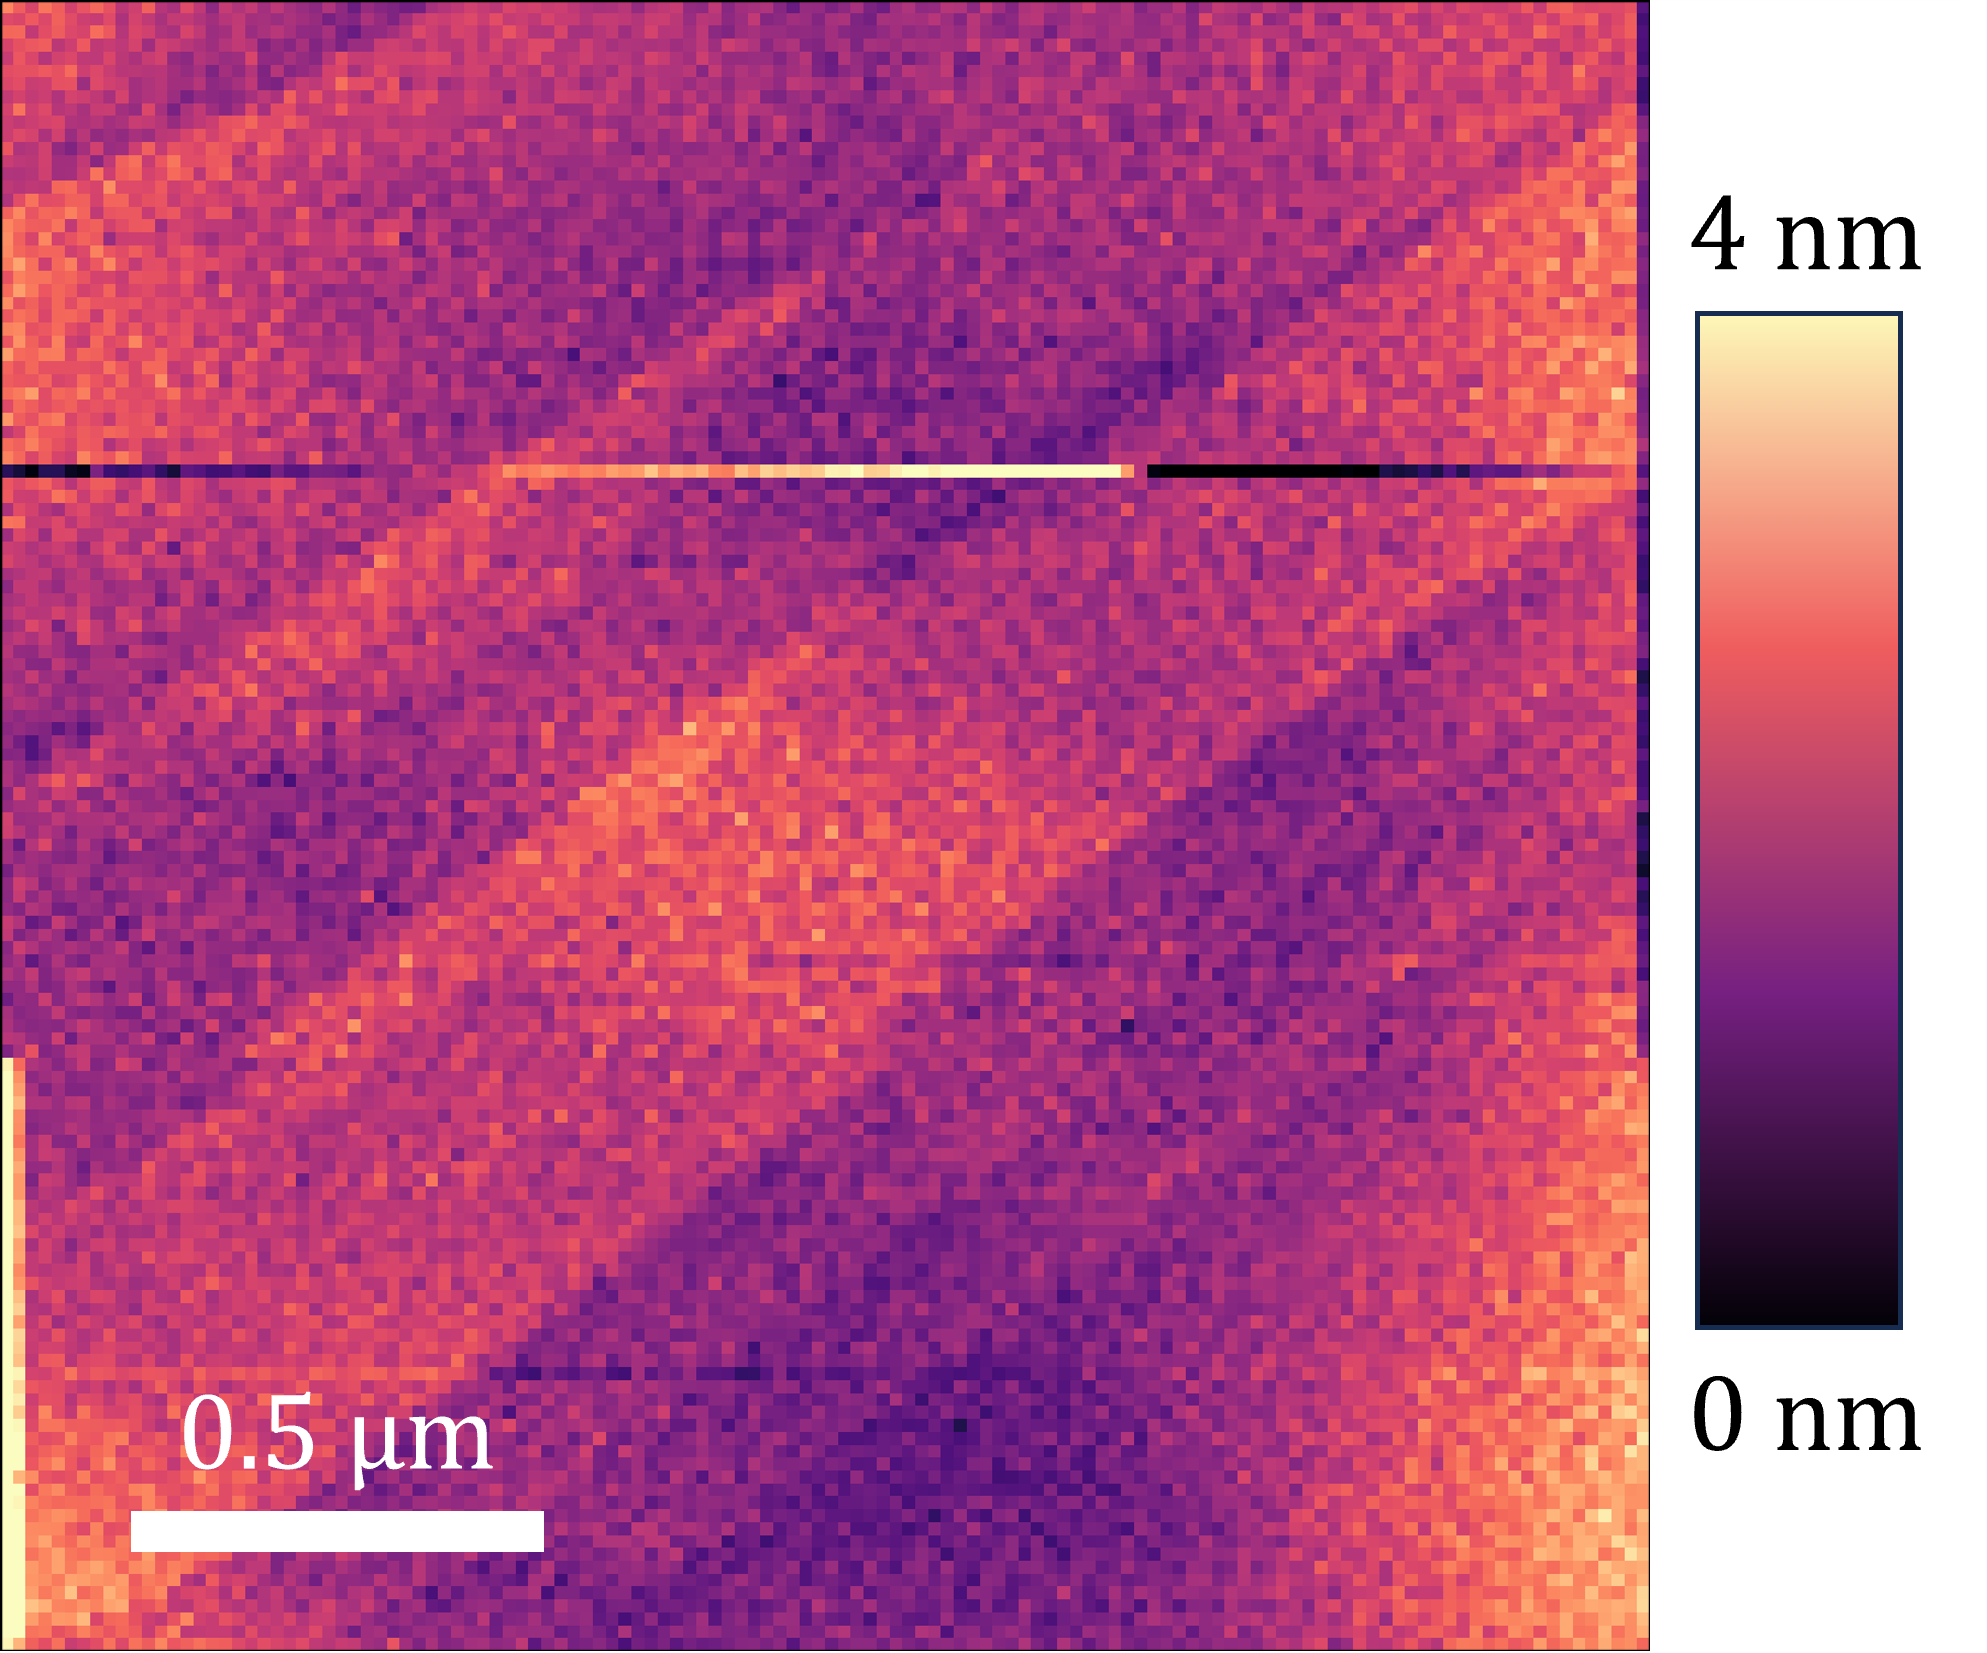
\includegraphics[width=0.6\linewidth]{figs/HOPG_strong_force.png}
  \caption{
    Height image acquired while the tip was strongly pressed against the surface, showing disappearance of the bubble-like feature and exposure of the underlying HOPG substrate.
  }
  \label{figS:HOPG_strong_force}
\end{figure}
\DIFaddbegin \ChangeTagEnd{r2_7_nanobubble_fit_si}\ChangeTagEnd{r2_6_tip_calibration_fit_si}
\DIFaddend 

\begin{figure}[p]
  \centering
  \DIFaddbeginFL 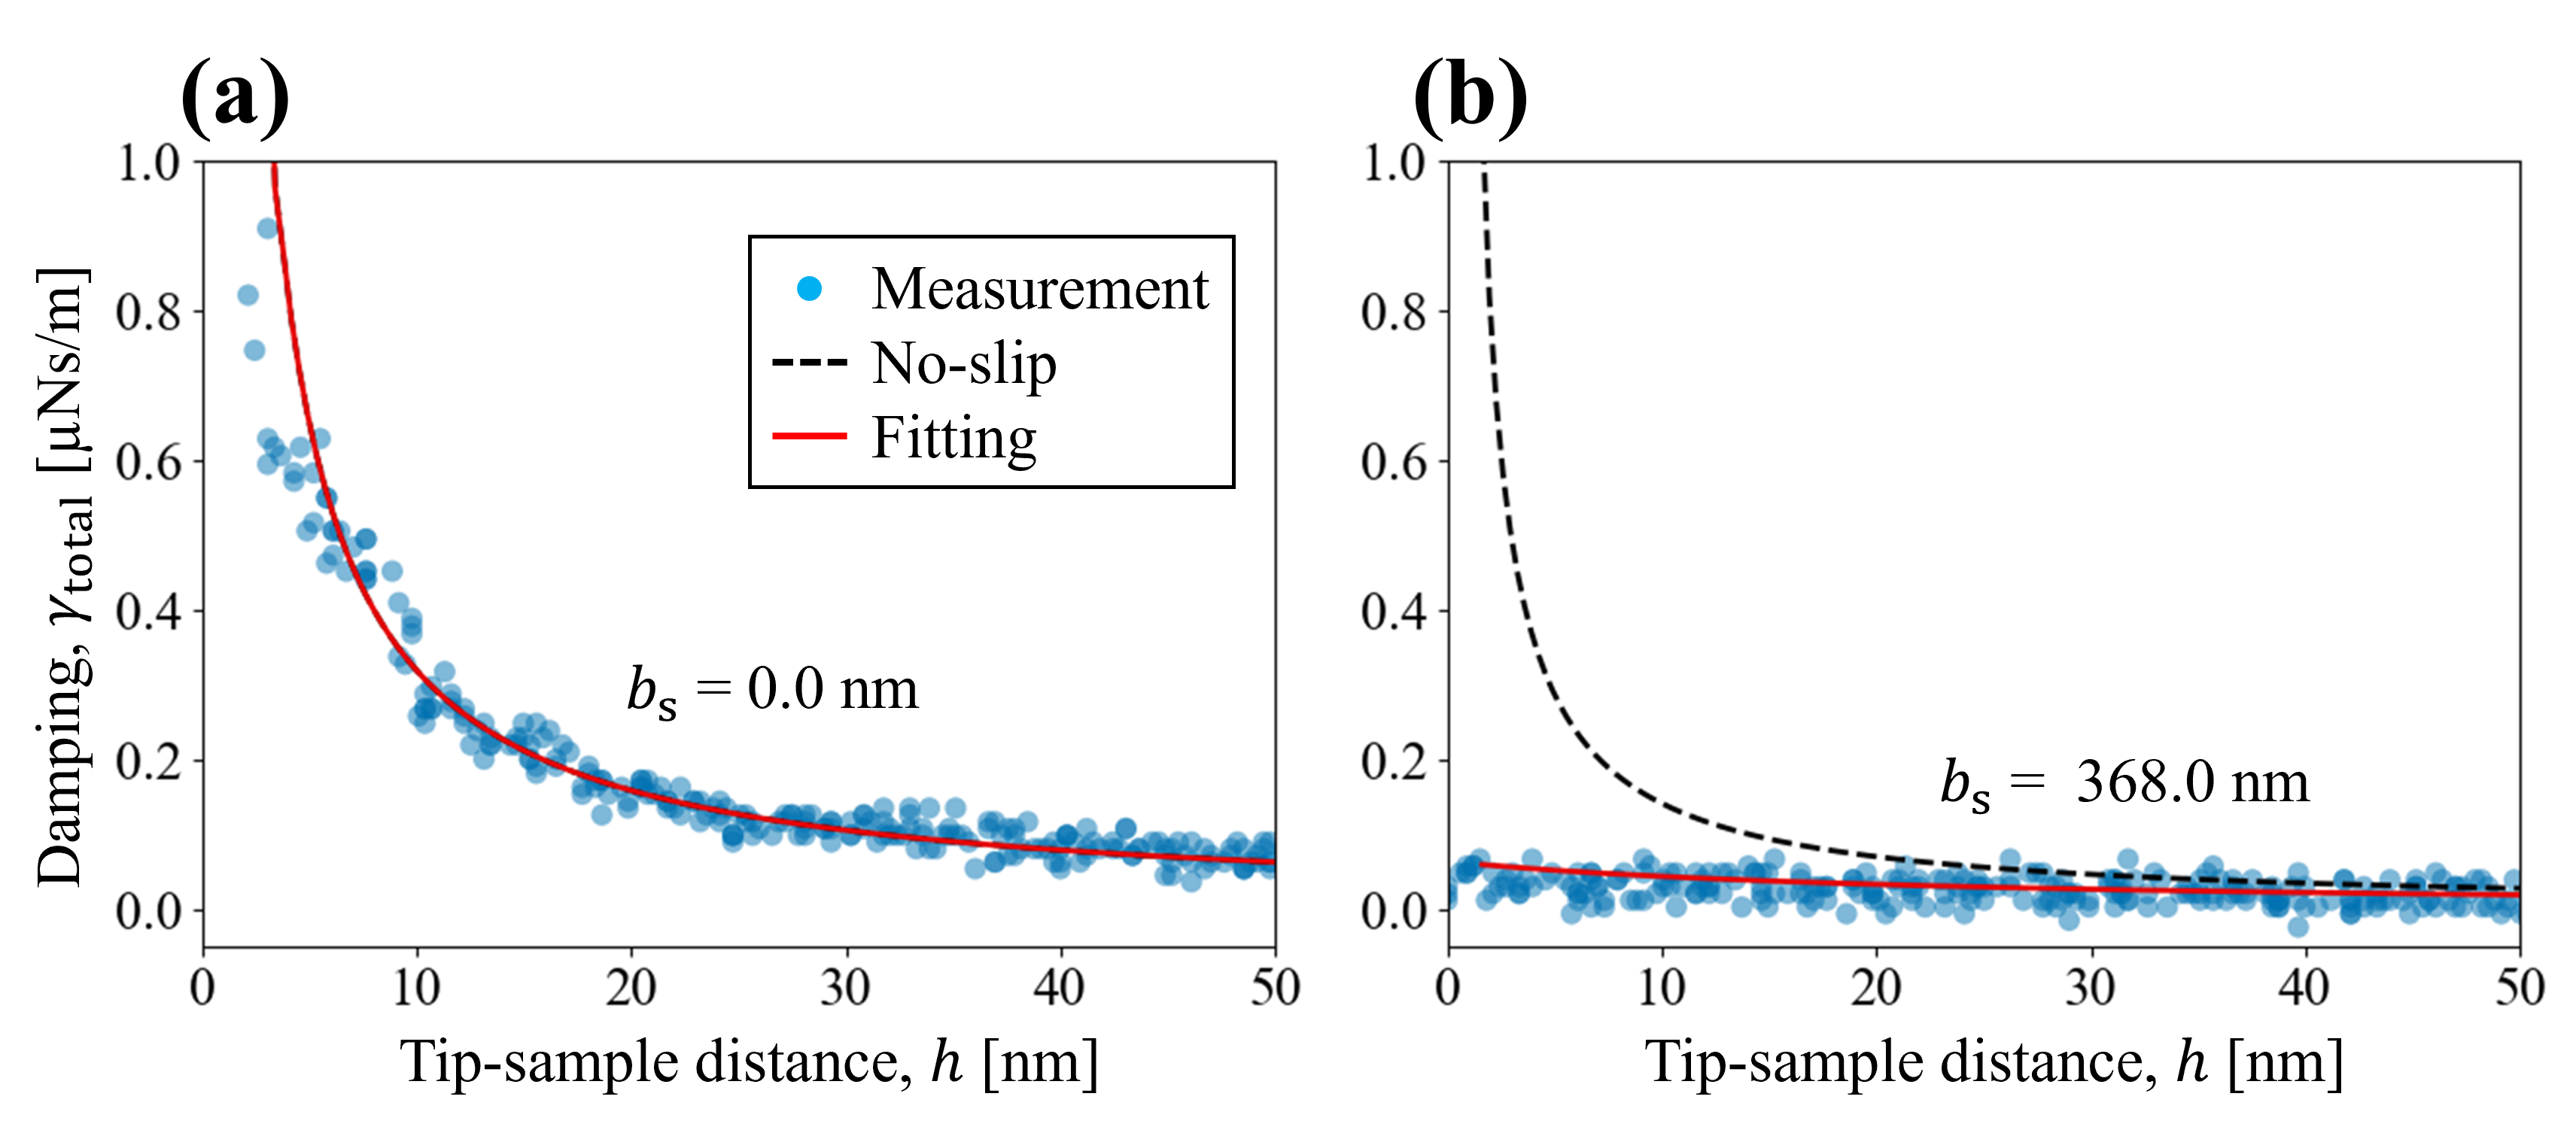
\includegraphics[width=1.0\linewidth]{figs/DLC_bubble.png}
  \caption{
    \DIFaddFL{Representative damping-coefficient fitting curves for (a) a atmospheric-plasma-treated DLC substrate and (b) a location above a nanobubble.
    The slip lengths shown in the panels were obtained from these representative single-point fits and therefore do not necessarily coincide with the mean values reported in the main text: \(0.0\pm1.2~\mathrm{nm}\) for DLC and \(345.3\pm23.7~\mathrm{nm}\) for nanobubbles.
    The mean absolute errors were \SI{0.016}{\micro\newton\second\per\metre} and \SI{0.014}{\micro\newton\second\per\metre} for (a) and (b), respectively.
  }}
  \label{figS:DLC_bubble_fit}
\end{figure}

\begin{figure}[p]
  \centering
  \DIFaddendFL 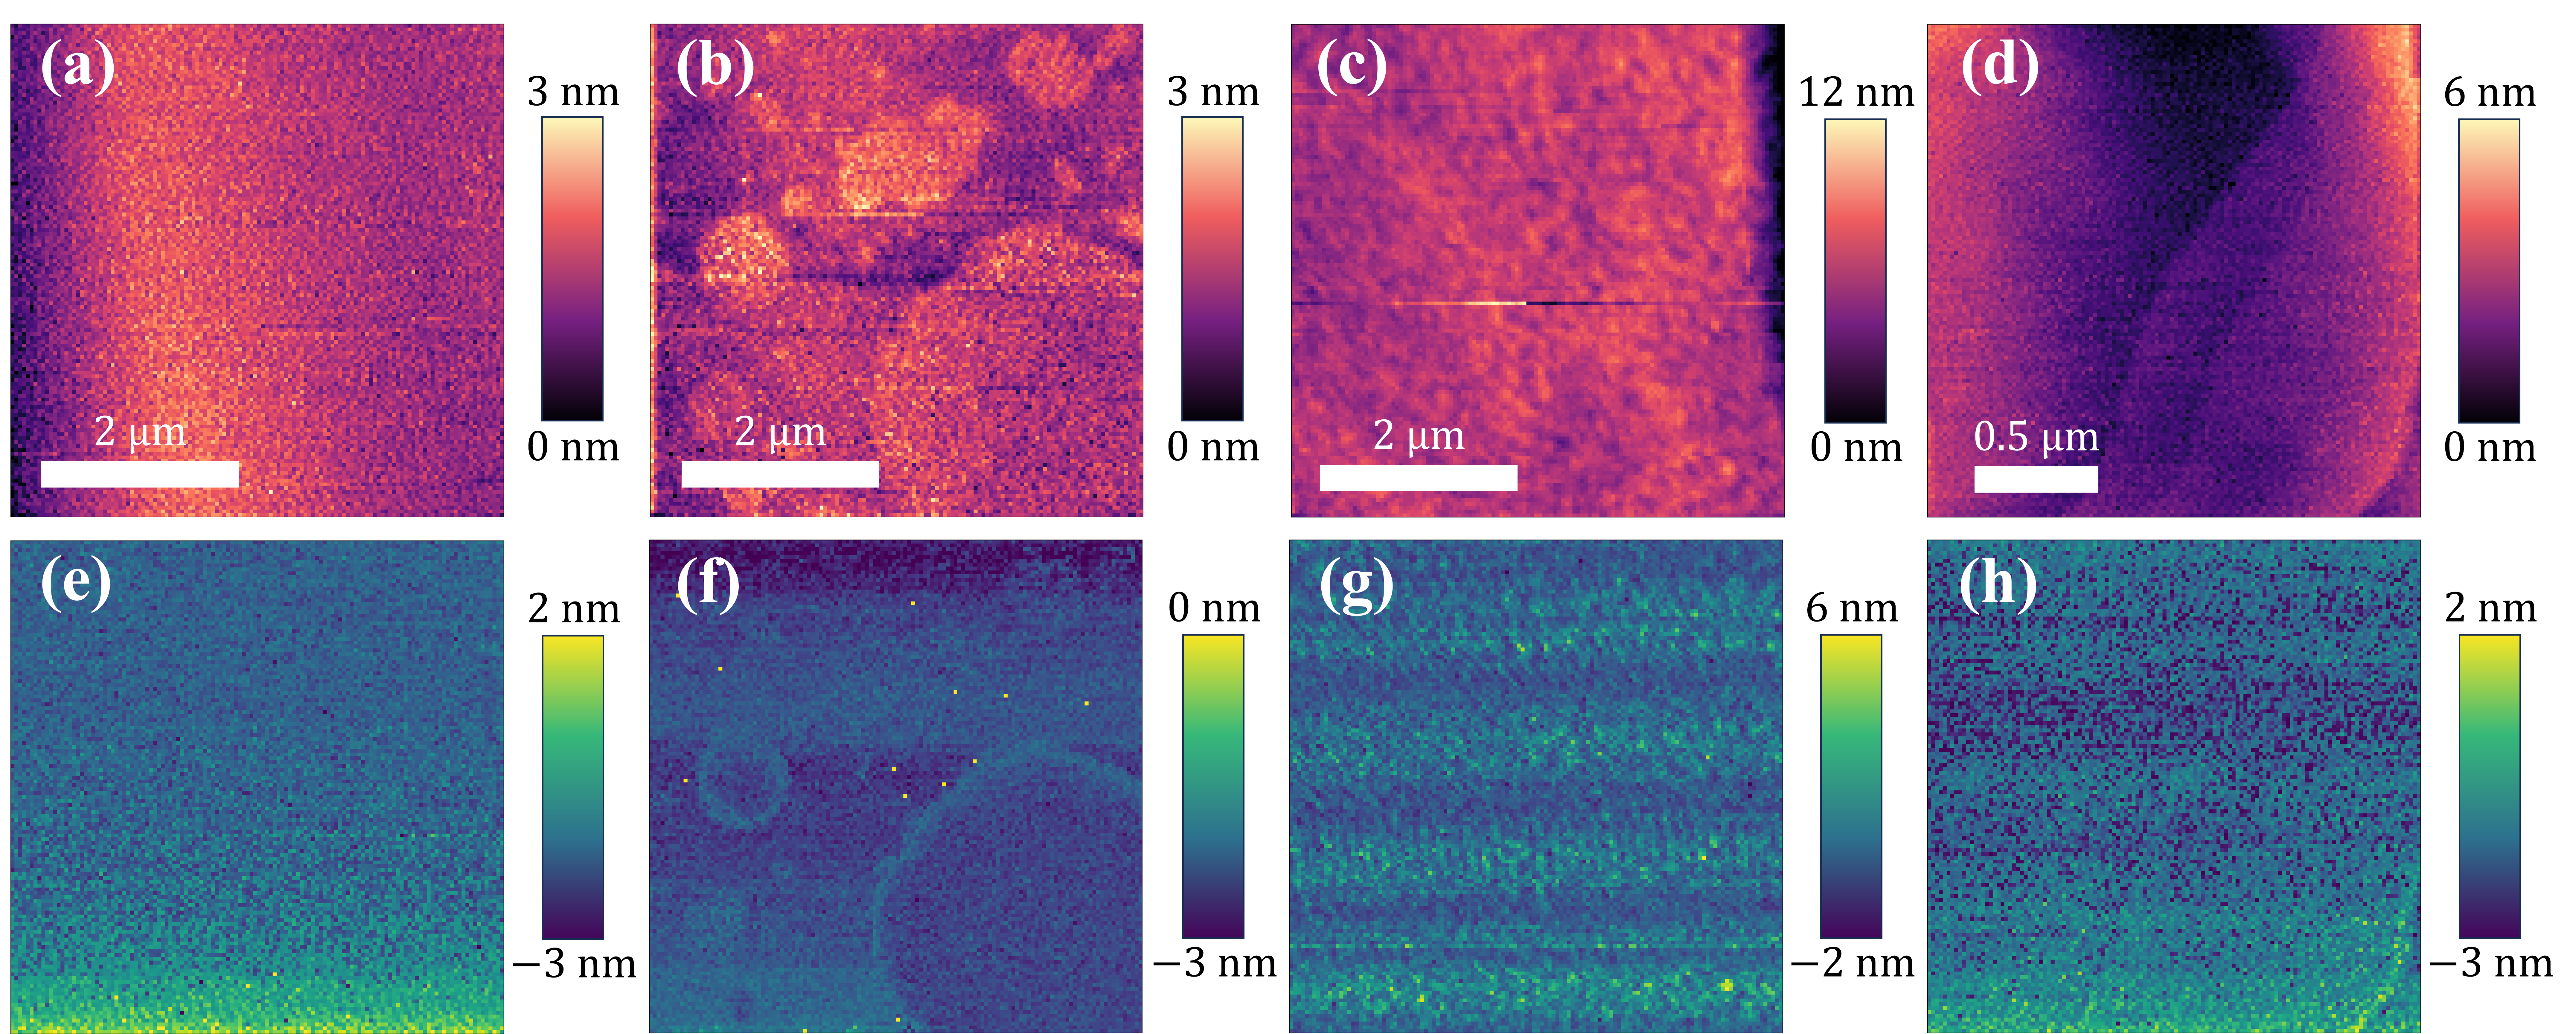
\includegraphics[width=1.0\linewidth]{figs/mapping_colormaps.png}
  \caption{ (a-d) Topography and (e-h) corresponding slip-length maps of (a, d) mica, (b, e) FDTS, (c, f) Teflon, and (d, h) HOPG. The \(R_a\) values were \SI{0.27}{\nano\metre}, \SI{0.29}{\nano\metre}, \SI{0.64}{\nano\metre}, and \SI{0.35}{\nano\metre} for each surface, respectively. Only the result for HOPG (d, h) was obtained in a \SI{10}{\milli\mole\per\litre} KCl solution and the others were in DI water.}
  \label{figS:mapping_colormaps}
\end{figure}

\DIFaddbegin \ChangeTagStart{r2_11_units_comparison_table_si}
\DIFaddend \begin{table}[p]
  \caption{Measured \DIFdelbeginFL \DIFdelFL{contact angles and }\DIFdelendFL slip lengths \DIFdelbeginFL \DIFdelFL{of }\DIFdelendFL \DIFaddbeginFL \DIFaddFL{and values calculated from Eq.~\ref{eqn:slip length scaling} for }\DIFaddendFL the substrates investigated in this study\DIFaddbeginFL \DIFaddFL{.}\DIFaddendFL }
  \label{tbl:contact_angle_slip}
  \DIFdelbeginFL %DIFDELCMD < \begin{tabular}{lcc}
%DIFDELCMD <     \hline
%DIFDELCMD <     %%%
\DIFdelFL{Substrate }%DIFDELCMD < & %%%
\DIFdelFL{Contact Angle \(\theta\) (\si{\degree}) }%DIFDELCMD < & %%%
\DIFdelFL{Slip length (\si{\nano\metre}) }%DIFDELCMD < \\
%DIFDELCMD <     \hline
%DIFDELCMD <     %%%
\DIFdelFL{Mica }%DIFDELCMD < & %%%
\DIFdelFL{\(< \SI{3}{\degree}\) }%DIFDELCMD < & %%%
\DIFdelFL{\(-1.7 \pm \SI{0.3}{\nano\metre}\) }%DIFDELCMD < \\
%DIFDELCMD <     %%%
\DIFdelFL{Oxygen plasma-treated silica }%DIFDELCMD < & %%%
\DIFdelFL{\SI{28.1}{\degree} }%DIFDELCMD < & %%%
\DIFdelFL{\(-0.7 \pm \SI{0.6}{\nano\metre}\) }%DIFDELCMD < \\
%DIFDELCMD <     %%%
\DIFdelFL{FDTS }%DIFDELCMD < & %%%
\DIFdelFL{\SI{97.9}{\degree} }%DIFDELCMD < & %%%
\DIFdelFL{\(-1.7 \pm \SI{0.2}{\nano\metre}\) }%DIFDELCMD < \\
%DIFDELCMD <     %%%
\DIFdelFL{FOPA }%DIFDELCMD < & %%%
\DIFdelFL{\SI{105.0}{\degree} }%DIFDELCMD < & %%%
\DIFdelFL{\(-0.9 \pm \SI{0.6}{\nano\metre}\) }%DIFDELCMD < \\
%DIFDELCMD <     %%%
\DIFdelFL{Teflon }%DIFDELCMD < & %%%
\DIFdelFL{\SI{111.1}{\degree} }%DIFDELCMD < & %%%
\DIFdelFL{\(0.8 \pm \SI{0.8}{\nano\metre}\) }%DIFDELCMD < \\
%DIFDELCMD <     %%%
\DIFdelFL{HOPG (DI water) }%DIFDELCMD < & %%%
\DIFdelFL{\SI{59.0}{\degree} }%DIFDELCMD < & %%%
\DIFdelFL{\(43.2 \pm \SI{5.8}{\nano\metre}\) }%DIFDELCMD < \\
%DIFDELCMD <     %%%
\DIFdelFL{HOPG (\SI{10}{\milli\mole\per\litre} KCl aq.) }%DIFDELCMD < & %%%
\DIFdelFL{\SI{62.8}{\degree} }%DIFDELCMD < & %%%
\DIFdelFL{\(-0.1 \pm \SI{0.7}{\nano\metre}\) }%DIFDELCMD < \\
%DIFDELCMD <     %%%
\DIFdelFL{HOPG (\SI{10}{\milli\mole\per\litre} NaCl aq.) }%DIFDELCMD < & %%%
\DIFdelFL{\SI{57.0}{\degree} }%DIFDELCMD < & %%%
\DIFdelFL{\(-2.3 \pm \SI{0.6}{\nano\metre}\) }%DIFDELCMD < \\
%DIFDELCMD <     \hline
%DIFDELCMD <   \end{tabular}
%DIFDELCMD < %%%
\DIFdelendFL \DIFaddbeginFL \centering
  \resizebox{\textwidth}{!}{%
  \begin{tabular}{lcccc}
    \hline
    Substrate & Contact Angle \(\theta\) (\si{\degree}) & Calculated \(b\), \(C = \SI{0.41}{\nano\metre}\) (\si{\nano\metre}) & Calculated \(b\), \(C = \SI{6.0}{\nano\metre}\) (\si{\nano\metre}) & Measured \(b\) (\si{\nano\metre}) \\
    \hline
    Mica & \(< \SI{3}{\degree}\) & \(\sim\SI{0.10}{\nano\metre}\) & \(\sim\SI{1.50}{\nano\metre}\) & \(-1.7 \pm \SI{0.3}{\nano\metre}\) \\
    Oxygen plasma-treated silica & \SI{28.1}{\degree} & \SI{0.12}{\nano\metre} & \SI{1.69}{\nano\metre} & \(-0.7 \pm \SI{0.6}{\nano\metre}\) \\
    FDTS & \SI{97.9}{\degree} & \SI{0.55}{\nano\metre} & \SI{8.06}{\nano\metre} & \(-1.7 \pm \SI{0.2}{\nano\metre}\) \\
    FOPA & \SI{105.0}{\degree} & \SI{0.75}{\nano\metre} & \SI{10.92}{\nano\metre} & \(-0.9 \pm \SI{0.6}{\nano\metre}\) \\
    Teflon & \SI{111.1}{\degree} & \SI{1.00}{\nano\metre} & \SI{14.65}{\nano\metre} & \(0.8 \pm \SI{0.8}{\nano\metre}\) \\
    HOPG (DI water) & \SI{59.0}{\degree} & \SI{0.18}{\nano\metre} & \SI{2.61}{\nano\metre} & \(43.2 \pm \SI{5.8}{\nano\metre}\) \\
    HOPG (\SI{10}{\milli\mole\per\litre} KCl aq.) & \SI{62.8}{\degree} & \SI{0.19}{\nano\metre} & \SI{2.83}{\nano\metre} & \(-0.1 \pm \SI{0.7}{\nano\metre}\) \\
    HOPG (\SI{10}{\milli\mole\per\litre} NaCl aq.) & \SI{57.0}{\degree} & \SI{0.17}{\nano\metre} & \SI{2.51}{\nano\metre} & \(-2.3 \pm \SI{0.6}{\nano\metre}\) \\
    \hline
  \end{tabular}
  }
\DIFaddendFL \end{table}
\DIFaddbegin \ChangeTagEnd{r2_11_units_comparison_table_si}
\DIFaddend 

%%%%%%%%%%%%%%%%%%%%%%%%%%%%%%%%%%%%%%%%%%%%%%%%%%%%%%%%%%%%%%%%%%%%%
%% The appropriate \bibliography command should be placed here.
%% Notice that the class file automatically sets \bibliographystyle
%% and also names the section correctly.
%%%%%%%%%%%%%%%%%%%%%%%%%%%%%%%%%%%%%%%%%%%%%%%%%%%%%%%%%%%%%%%%%%%%%
\clearpage
\bibliography{main}

\end{document}

